\documentclass{sig-alternate}
\usepackage{verbatim}
\usepackage{array}
\usepackage{caption}
\usepackage{subcaption}
\usepackage{amsmath}
\usepackage{amssymb}
\usepackage{graphicx}
\captionsetup{compatibility=false}

\DeclareMathOperator*{\argmin}{arg\,min}


\begin{document}

\author{}
%\author{Craig Willis \and Garrick Sherman \and Miles Efron}

\CopyrightYear{2016} 
\conferenceinfo{ASIST '16,}{October 14 - 18, 2016, Copenhagen, Denmark}

\title{What makes a query temporally sensitive?}

\maketitle


\begin{abstract}

This work examines factors that affect manual classifications of ``temporally sensitive'' information needs.  We introduce the concepts of \emph{temporal relevance} and \emph{temporal topicality} to differentiate between different aspects of temporal retrieval research. We use qualitative and quantitative techniques to analyze 660 topics from the Text Retrieval Conference (TREC) previously used in the experimental evaluation of temporal retrieval models.  Regression analysis is used to model previous manual classifications. We identify factors and potential problems with previous classifications, proposing principles and guidelines for future work on the evaluation of temporal retrieval models. 

\end{abstract}


\section{Introduction}

A growing body of information retrieval research argues that temporality should be modeled explicitly when scoring and ranking documents with respect to users' queries. Time-related criteria such as recency, currency, and freshness have long been recognized as factors in studies of relevance \cite{Barry1998, Mizzaro1997, Dai2010, Dong2010}. Based on these criteria, researchers have explored a variety of temporal retrieval models that explicitly incorporate time into document rankings \cite{Li2003,Efron2011,Dakka2012,Kanhabua2011,Kanhabua2012a,Peetz2013a}. Researchers often refer to general classes of ``temporal queries'' or ``temporal information needs.''  Models have been proposed for ``recency queries'' \cite{Li2003,Efron2011}, ``time-sensitive queries'' \cite{Dakka2012}, ``implicitly temporal queries'' \cite{Metzler2009}, and ``temporally biased queries'' \cite{Jones2007}.  For evaluation,  these studies rely on manual classifications of topics into temporal categories and standard test collections with documents and associated relevance judgements.

In this paper, we take a deeper look into these manually classified topics to develop a clearer understanding of \emph{what makes a query temporally sensitive}?  Previous manual classifications combine the temporal distribution of judged-relevant documents with common-sense notions of topic temporality often without a clear explanation of the criteria or processes used for classification. Since the processes being modeled are unclear, using these manually classified topics for evaluation is of questionable value. 

To address our main question, we analyze  660 topics from the Text Retrieval Conference (TREC) previously used in the experimental evaluation of temporal retrieval models. We employ content analysis to identify topic characteristics that might affect the manual assessment of ``temporal-sensitivity.'' The resulting coded topics are used in a set of regression analyses to assess the relationships between these characteristics and manually assigned categories.   This paper's main contribution is an in-depth, empirically based assessment of the complexities that underpin temporal IR.  This assessment helps us understand earlier temporal IR studies, explaining the difficulty in using existing test collections for evaluation, while also suggesting novel ways to incorporate time effectively into retrieval.

\section{Temporality and IR Test Collections}

\subsection{TREC topics}

Test collections developed for TREC generally consist of a collection of documents, a set of topics and associated relevance judgments. Document collections may be from a single source (e.g., Microblog) or composed of multiple sub-collections with distinct start and end dates (e.g., TREC8, KBA).  Although the methods of creation have changed over time, TREC topics are generally intended to mimic real users' information needs with respect to the underlying document collection and typically include a \textit{title} (similar to a keyword query) and a \textit{description} (one or two sentences about the information need) \cite{Voorhees2005}.   Topics are created in the context of a particular document collection and documents' relevance judgements are made by assessors for topic/document pairs.

Many temporal information retrieval models have be evaluated using existing TREC topics and test collections \cite{Li2003, Jones2007, Efron2011, Dakka2012, Peetz2013a}. Since the original collections do not contain information about query temporality, researchers have manually assigned temporal categories  based on topic titles and descriptions.  A central goal of these earlier studies is to discover information available but overlooked in these existing collections.


\subsection{Time and relevance}

There are numerous notions of temporality in information retrieval research, each of which requires different methodologies for analysis. In this study, we are primarily concerned with what we call a query's \emph{temporal relevance}: the extent to which relevant documents' publication times follow a non-uniform distribution. We distinguish this from \emph{temporal topicality} which refers to information needs that are satisfied by documents about certain periods in time. Of course, an information need may combine the two conditions. Examples of studies concerned with temporal topicality include \cite{Berberich2010,Kanhabua2011}. These can be further differentiated from \emph{temporal query dynamics}, which explores  queries over time \cite{Shokouhi2011,Kulkarni2011} often independent of the underlying document collection.

\subsection{Time-sensitive queries}

In this section, we review examples of studies focused on \emph{temporal relevance}.  The list of topics and collections used in each of the studies are listed in Table \ref{table.topics}. 

\begin{table*}
\small
\resizebox{\textwidth}{!}{%
\begin{tabular}{| p{2cm} | p{6cm}  | p{6cm} |} \hline
\bf{Topics} & \bf{Collections} & \bf{Studies}\\ \hline
51-200 & TREC Disks 1-2 AP (1988-89) & Jones \& Diaz (2007) \\ \hline
301-450 &  TREC Disks 4-5 FT (1991-94) \newline LA Times (1988-89) & Efron \& Golovchinsky (2011); \newline  Dakka, Gravano \& Ipeirotis (2012) \\ \hline
N1-100 & AQUAINT Xinhua (1996-2000)\newline NYT (1999-2000) & Jones \& Diaz (2007) \\ \hline
851-1050 & Blog06  (Dec 6, 2005 - Feb 21, 2006) & Peetz, Meij \& de Rijke (2013) \\ \hline
MB1-110 & Tweets 2011 (Jan 24, 2011 - Feb 8th, 2011) & Efron, Lin, de Vries (2014)\\ \hline
\end{tabular}}
\caption{TREC topics and Collections Used in Prior Temporal Retrieval Studies.}
\label{table.topics}
\end{table*}

Li and Croft's study of ``recency queries''  \cite{Li2003} was among the first to address temporal relevance. Li and Croft hypothesize that some queries are ``recency queries'' where recently published documents have a high \textit{a priori} probability of relevance.  Through the direct analysis of the temporal distribution of judged relevant documents, they classify a subset of queries as recency queries because they have ``more relevant documents in the recent past.''

Jones and Diaz \cite{Jones2007} study the temporal characteristics of queries with the goal of query classification through the analysis of three TREC news collections and a web search engine log. They define three classes of queries based on the manual analysis of topics: temporally ambiguous (requesting multiple events),  temporally unambiguous (requesting a single event), and atemporal (having no preference). Jones and Diaz manually classify 100 TREC topics based on title, description, and narrative fields. Specific criteria for classification are not given. For the AP and WSJ collections, they find that all of the queries are either atemporal or temporally ambiguous. For increased diversity, they add the 2003 Novelty track topics because they include topics classified as ``event'' or ``opinion,'' which the authors suggest correspond to the ``temporally unambiguous'' and ``atemporal'' categories, respectively.

Dakka, Gravano, and Ipeirotis  \cite{Dakka2012} investigate a broader class of queries which they refer to as ``time-sensitive.'' They hypothesize that there are queries for which more relevant documents are found at specific points in time, not just recently. They manually examine the title, description and narrative of each topic and identify queries associated with specific news events. In cases where the topic information is insufficient to make a decision, they analyze the distribution of judged-relevant documents. The resulting classification consists of 86 temporally sensitive queries. 

Efron and Golovchinsky \cite{Efron2011} investigate additional models for recency queries.  Topics are classified as ``recency'' if at least 2/3 of the relevant documents occur after the median document time and the topic has a ``bona fide temporal dimension'' based on manual review, the specific criteria for which are not specified.  

Finally, Peetz, Meij, and de Rijke \cite{Peetz2013a} investigate the effect of temporal bursts in estimating query models. Building on the earlier studies, they evaluate their models using the above test collections as well as a new collection based on TREC Blog06. As in the previous studies, the authors construct a subset of ``temporal'' queries through manual evaluation of topic descriptions and relevant document distributions. No specific criteria for classification are given.

In each of these studies, which are central to the work presented here, the authors manually classify queries from existing test collections into temporal categories. For each study, we have a known test collection consisting of a set of documents, queries, relevance judgements, and temporal classifications.  


\subsection{What makes a query temporally sensitive?}

Given the complex landscape described in the previous section, what in general makes a query temporally sensitive? Dakka et al \cite{Dakka2012} present a compelling definition. A query is ``time sensitive''  if  ``the relevant documents for the query are not spread uniformly over time, but rather tend to be concentrated at restricted intervals.''  In other words, a query is temporally sensitive if relevant documents are more likely to occur at some points in time than others. This is an essential point, since many temporal retrieval models rely on the temporal distribution of results in document scoring. However, the distribution of relevant documents alone is not sufficient to determine true temporality (non-uniformity of document distributions with respect to time can be due to many factors). To address this, most of the studies listed above rely on common-sense notions of temporality based on the topic content considered independently of the distribution of relevant documents. Dakka et al refer to ``newsworthiness''; Efron and Golovchinksy to a ``bona fide temporal dimension''; and Jones and Diaz to ``events.''  A primary goal of the current study is to look deeper into these common-sense criteria with the aim of providing researchers a firmer basis for assessing which queries are likely to have a \emph{temporal relevance} dimension.


\subsection{Other related test collections}

This study is concerned with the analysis of manually classified queries as they relate to the concept of \emph{temporal relevance}. This study is also limited to queries used in ad-hoc retrieval and does not address those used in filtering tasks such as the recent Knowledge Base Acceleration (KBA) \cite{Frank2013} and Temporal Summarization \cite{Guo2013} tracks.  While certainly pertinent to the investigation of query temporality, the topics and test collections used in these tracks are concerned with long standing and prospective information needs and are therefore fundamentally different from those used in ad-hoc studies. 

In the case of KBA, topics are represented as named-entities in a knowledge base (e.g., Wikipedia). The task is to recommend edits to the knowledge base entity from a timestamped stream of documents.  Little information is given about why the entities were selected, although we can assume from the task that some entities were selected because new information is received about them over the timeframe of the corpus. 

Similarly, the Temporal Summarization track is concerned with ``online updating of time-critical events'' \cite{Guo2013}. While we can again assume from the task that each topic is time-critical and therefore temporal, the test collection lacks any explicit manual classifications of topic temporality.  Also, since the track is concerned with online updating, the relevance assessments are quite different from those in previous ad-hoc studies.

We also do not include the topics developed for the NTCIR Temporalia test collection \cite{Joho2014} because they diverge from our definition of \emph{temporal relevance}.  Both the Temporal Query Intent Classification (TQIC) and Temporal Information Retrieval (TIR) test collections contain queries explicitly classified into four categories: past, recency, future, and atemporal. On the surface, these categories seem to relate to those discussed above. However, further inspection reveals that the queries in these test collections are primarily concerned with \emph{temporal topicality}.  
We'll use an example to illustrate the distinction between \emph{temporal topicality} and \emph{temporal relevance} in the Temporalia collection. 

The authors provide the example topic about the film ``Girl with the Dragon Tattoo'' in the context of four temporally-categorized questions:

\begin{itemize}
\item Past: How did the casting of the film develop?
\item Recency: What did the recent reviews say about the film?
\item Future: Is there any plan about its sequel?
\item Atemporal: What are the names of main actors and actresses of the film?
\end{itemize}

In this example, ``How did the casting of the film develop?'' is a question \emph{about} the past. Using our definition of \emph{temporal relevance}, a query concerned with the past would have more relevant documents in the past. However, we can imagine that a recent document discussing the historical development of casting for the film would be highly relevant to this information need. Similarly, there can be no ``future'' in \emph{temporal relevance} since it is not possible to have relevant documents in the future. It is, however, possible to have relevant documents \emph{about} the future, as with the question ``Is there any plan about its sequel.''

Additionally, the TQIC collection does not include relevance judgments, so it not possible to relate the manual classifications to distributions of judged-relevant documents. Based on this, we have found that the NTCIR test collections are not well-suited for an analysis of \emph{temporal relevance}.

These test collections are discussed here, but not included in the analysis presented in this paper.


\section{Methods}

In the studies reviewed in Section 2.3, researchers rely in part on existing TREC test collections to evaluate proposed temporal retrieval models. In each study, topics are manually categorized (e.g.,  temporal or non-temporal) to assess model performance. This study further investigates the characteristics of topics deemed temporal. To achieve this, we use a combination of qualitative content analysis and regression analysis, as described below.

\subsection{Qualitative coding}
We use content analysis \cite{Krippendorff1980} to identify characteristics of TREC topics potentially associated with temporal sensitivity. 660 topics were selected from the TREC Ad-hoc, Novelty, Blog, and Microblog tracks. These topics have previously been used by researchers to evaluate temporal retrieval models. They have associated, published manual classifications or are from collections with known temporal characteristics (i.e., Microblog). The complete set of topics used in this study are listed in Table \ref{table.topics} along with the temporal constraints of each collection or sub-collection.



Two of the authors participated in the development of the codebook and subsequent coding of topics. Codebook development began with a preliminary reading of all topic titles, descriptions and narratives. Codes were defined based on characteristics of topics expected to be related to temporal sensitivity, informed by the literature. Of the 660 topics, 330 were coded by both coders to allow for inter-rater consistency analysis. During this process, code definitions were refined and clarified. In the final coding, only topic title and description were used. The final codebook is presented in Table \ref{table.codebook}. Coding was completed using the Dedoose\footnote{http://www.dedoose.com} service.  After coding all 660 topics, the topic/code matrix was exported for subsequent reliability and regression analysis, as described in the following sections. 

\begin{table*}[!ht]
\small
\resizebox{\textwidth}{!}{%
\begin{tabular}{| p{2cm} | p{9cm}  | p{4cm} |} \hline
\bf{Code} & \bf{Description} & \bf{Examples}  \\ \hline
Specific Event & Something significant that happens at a specific time and place. Code title and description in concert, even if title does not contain event specifics. & Mount Pinatubo erruption on June 15, 1991; 2008 State of the Union; Hurricane Hugo \\ \hline
Generic Event & Use this code when the topic refers to more than one specific event or a class or type of event. Only use this code if every instance of the event type would be newsworthy (i.e., a specific event) and the central topic of a news article. & Earthquakes, volcano erruptions, elections, disputes, strikes \\ \hline
Indirect Event Reference & Apply this code to indicate when the topic might be indirectly referring to a *specific* event. Use only if you need to turn to external information to identify potential specific events (e.g., your personal knowledge, wikipedia). Do not use if specific event information is contained in the description. & Legally assisted suicide, related to Kevorkian controversy. Partial birth abortion ban, related to partial birth abortion ban legislation. Surrogacy related to Baby M. \\ \hline
Periodic Event & Apply this code to indicate when an event is periodic, recurring at regular, predictable intervals. Never double-code as SpecificEvent or as an entity even though periodic events are often named entities. & Super bowl, Nobel awards, Oscars, State of the Union \\ \hline
FutureEvent & Apply this code to indicate when a topic refers to a future predicted specific event. Never double-code as SpecificEvent. & 2020 Fifa, 2016 Summer Olympics \\ \hline
Person Entity & Apply this code to identify personal names in topics. & President Bush; Sasha Cohen;  \\ \hline
Place Entity & Apply this code to identify places in topics. Limit to proper names. Also apply to references to nations, governments or government bodies. & Peru; Africa; African; European; Atlanta \\ \hline
Organization Entity & Apply this code to identify organizations in topics. Limit to proper names. Do not apply to references to governments (e.g., United States), use PlaceEntity instead. & Hitachi Data Systems; U.S. Congress; \\ \hline
Other Entity & Apply this code to named entities that are not people, places or organizations. Limit to proper names. Includes movies, books., etc. & Hubble Telescope; The Avengers; Euro	\\ \hline
Explicit Date & Apply this code to identify explicit dates. & 1988; June 15, 1991; October 2007; Monday \\ \hline
\end{tabular}}
\caption{Codebook}
\label{table.codebook}
\end{table*}


An example of a coded topic from the 2004 Novelty test collection is presented in Figure \ref{fig.example}.  This topic refers to a specific event and contains place entities as well as an explicit date.  Topic N57 is categorized as an ``event'' by the TREC topic creator and is therefore an unambiguous temporal topic as defined by Jones and Diaz.

\begin{figure}[!ht]
\begin{equation*}
\begin{split}
\mbox{\bf{Title}:} & \big[(\mbox{East Timor})_{PlaceEntity} \\
	& \mbox{Independence}\big]_{SpecificEvent} \\
\mbox{\bf{Description}:} & \big[  (\mbox{East Timor})_{PlaceEntity} \\
	& \mbox{ vote for independence from } \\
	& (\mbox{Indonesia})_{PlaceEntity} \mbox{ in } \\
	& (\mbox{August 1999})_{ExplicitDate}\big]_{SpecificEvent}
\end{split}
\end{equation*}
\caption{TREC Novelty 2004 topic N57 example annotation}
\label{fig.example}
\end{figure}

In addition to coding the topics based on the defined codes, the coders assigned a temporal designation to the distribution of relevant documents for each topic. This was a subjective process to determine whether there is agreement about topic-temporality based strictly on the ``shape'' of the distribution of relevant documents. Non-parametric densities were fit to the temporal distribution of relevant documents for topics with more than 20 relevant documents, following Dakka et al. Each coder reviewed the relevant document distribution along with the total number of relevant documents for each topic and assigned one of four values based on subjective impressions about the degreee to which relevant documents were temporally constrained:  too few observations (-1), low or no temporality (0), moderate temporality (1), and high temporality (2). 
\subsection{Reliability analysis}

For this study, coder agreement is measured using Cohen's $\kappa$ for the classification of the distribution of relevant documents. For the broader qualitative coding task, we use a variation of percent overlap, since coding is performed on arbitrary segments of text. We define the \emph{percent overlap} as:

\[
overlap = \frac{m}{m + u_1 + u_2} 
\]

Where $m$ is the number of excerpts assigned the same code by both coders, $u_1$ is the number of codes assigned to excerpts only by coder 1 and $u_2$ is the number of codes assigned to excerpts only by coder 2. If both coders assign no codes to a topic, it is considered perfect agreement. We report the macro (calculated over all topics) and micro (calculated as a per-topic average) overlaps.  Per-code overlaps are used to characterize coder agreement within each code.

\subsection{Relevant document distributions}

In each of the four prior studies enumerated in Section 2.3, the original authors acknowledge using the distribution of judged-relevant or pseudo-relevant documents in determining topic temporality. For this study, we use two different measures to represent these distributions: the first-order time series autocorrelation (ACF) and the dominant power spectrum (DPS).

Jones and Diaz \cite{Jones2007} use the ACF created by the temporal distribution of pseudo-relevant documents for a query as a predictor of query temporality. They note that queries with strong inter-day dependencies will have high ACF values, indicating predictability in the time series. The first-order autocorrelation of the time series $X$ is defined by Equation \ref{eq.acf}:

\begin{equation}
r_1 = \dfrac{\sum_{i=1}^{N-1} (x_t - \bar{x}_{(1)})(x_{t+1} - \bar{x}_{(2)})}{ \big [ \sum_{i=1}^{N-1}  (x_t - \bar{x}_{(1)})^2 \big ] ^{1/2} \big [\sum_{i=1}^{N-1} (x_{t+1} - \bar{x}_{(2)})^2 \big ]^{1/2}}
\label{eq.acf}
\end{equation}

Similarly, He, Chang, and Lim \cite{He2007} use the DPS as a predictor of the ``burstiness'' of temporal features for event detection. The DPS is the highest power spectrum, estimated using the periodogram. The periodogram is the sequence of the squared magnitude of the Fourier coefficients $\Vert X_k \Vert^2$ indicating the signal power at frequency $k/T$ in the spectrum.  The discrete Fourier transform is defined by Equation \ref{eq.dps}:
\begin{equation}
X_k = \sum_{t=1}^T y_f(t)e^{\frac{2\pi i}{T}(k - 1)t}, t=1,2,....T
\label{eq.dps}
\end{equation}

In this study, both ACF and DPS measures are used to reduce the distribution of judged-relevant or pseudo-relevant documents to a single value for the regression analysis, as described in the next section.

\subsection{Regression analysis}

% ??? I assume that topics deemed to have too few rel docs (i.e. -1 codes) were omitted, right?  Maybe say that for clarity wrt the response variable of the model.
A primary goal of this study is to determine the characteristics that contribute to the manual judgment of topic temporality. We use logistic regression based on the generalized linear model (GLM) implementation in R. The predictors are binary presence indicators for each of the qualitative codes along with the ACF and DPS of the temporal distribution of true-relevant documents.  The response variables are the binary temporal/non-temporal indicators manually assigned in the four studies.  Model variables are selected using standard step-wise procedures based on the Akaike information criterion (AIC). Coefficients are reported using the log-odds and model fit is assessed using pseudo-$R^2$.

\section{Results}

% In this section we report the results of our analysis including a summary of the qualitative codes and their distributions, coder agreement/reliability, and regression models. We also report the results of the comparison between the manual assessment of the relevant document distributions and the ACF and DPS values.

\subsection{Codes}

Our qualitative analysis suggests that three broad classes of features bear on query temporality: events, named entities, and explicit dates. It is intuitive that topics focused on specific and important events will have a higher degree of temporal relevance. Perhaps the most essential code is the ``SpecificEvent'' -- something important that happens at a particular time and place.  This follows the Topic Detection and Tracking (TDT) definition \cite{TDT2004} of ``seminal events'' that happen at specific times in specific places, often to individuals or other named entities (e.g., organizations).  Related to SpecificEvent is the ``PeriodicEvent,'' which refers to an event that recurs periodically, such as the Super Bowl, World Cup, or Halloween. Jones and Diaz \cite{Jones2007} note that many of the early ad-hoc queries were temporally ambiguous, referring to multiple events. We incorporate this concept through the ``GenericEvent'' code, which captures topics concerned with a class of specific events, such as earthquakes, elections, or strikes, but not a specific instance of these events.  While analyzing the topics, it became apparent that some topics were likely to be inspired by a specific event, but without explicit reference in the topic description. This concept is captured through the ``IndirectEventReference'' code. 
 
 
The remaining codes are concerned with the identification of specific types of named entities, which are expected to have some  association with topic temporality, and explicit dates.


\subsection{Code distributions}

Figure \ref{fig.codedist} summarizes the percent of topics in each test collection with each code assigned. We can see that the Novelty and Microblog  collections have a higher percentage of specific events than the Blog and other ad-hoc collections. The earlier ad-hoc collections have a higher number of generic events, which confirms the findings of Jones and Diaz \cite{Jones2007}. The Blog, Novelty, and Microblog test collections each have larger numbers of named entities in the topic titles and descriptions.

\begin{figure*}[!ht]
\centering
\begin{subfigure}{.5\textwidth}
  \centering
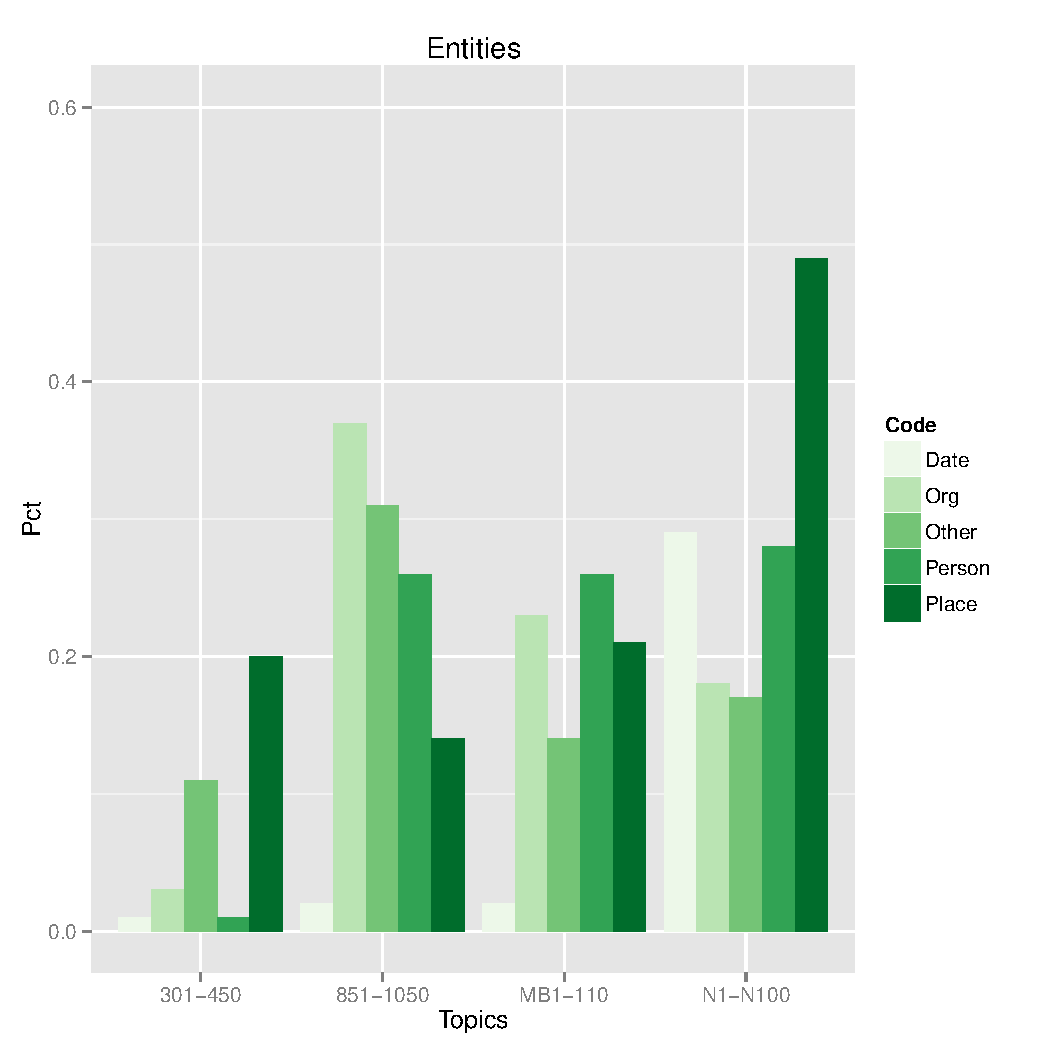
\includegraphics[width=8cm, height=6cm]{plots/topic-groups-ent.pdf}
\end{subfigure}%
\begin{subfigure}{.5\textwidth}
  \centering
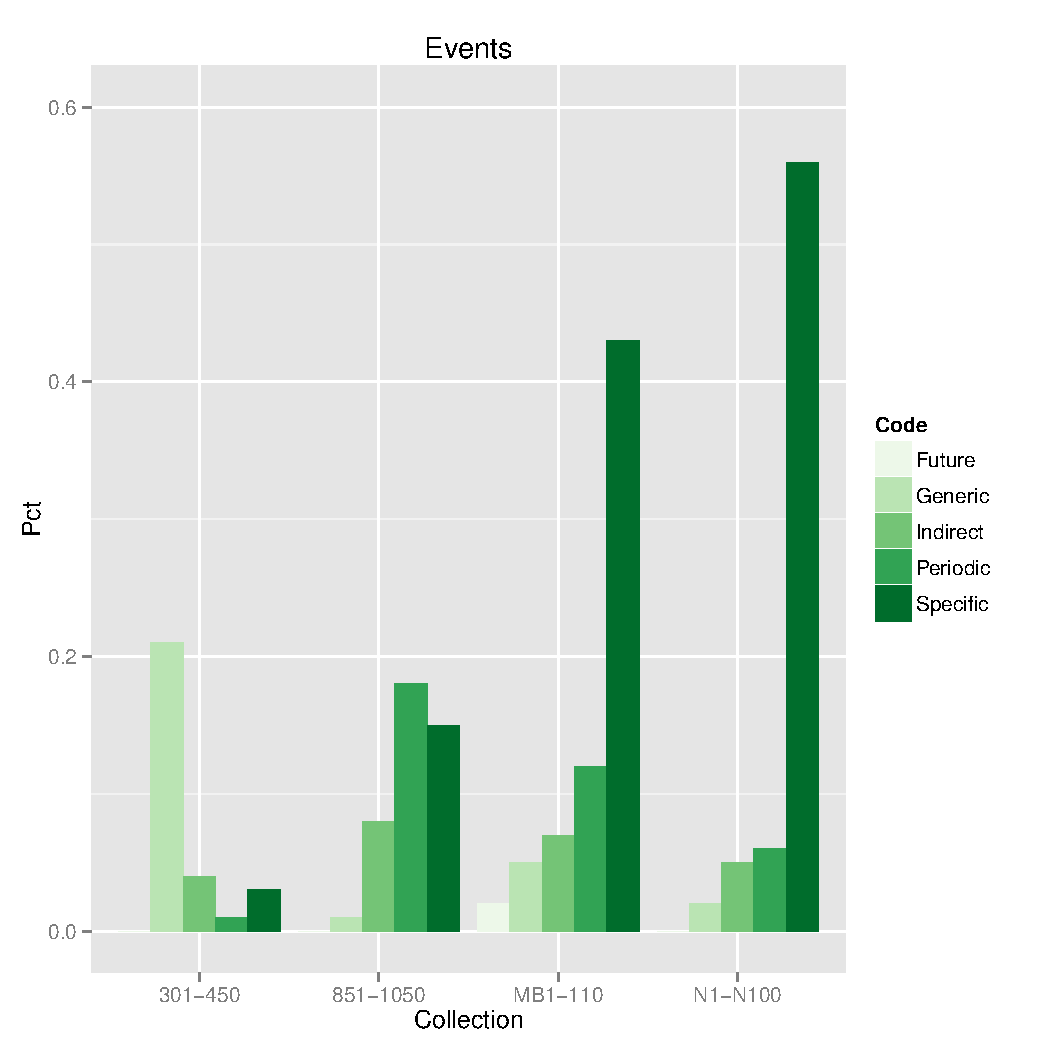
\includegraphics[width=8cm, height=6cm]{plots/topic-groups-evt.pdf}
\end{subfigure}
\begin{subfigure}{\textwidth}
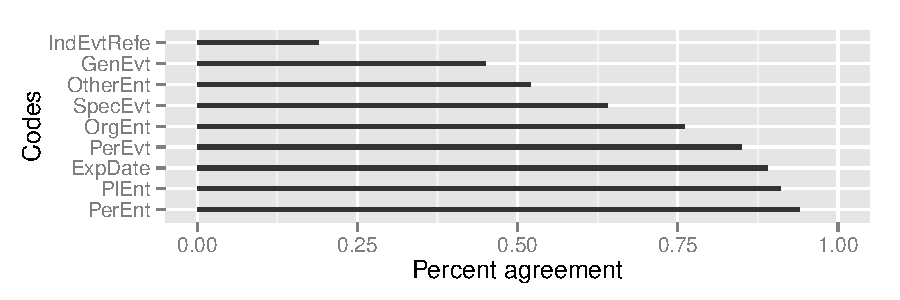
\includegraphics[width=17cm]{plots/coder-agreement.pdf}
\end{subfigure}
\caption{Percent of topics in each collection with codes assigned from the (a) entity code group and (b) events code group; (c) percent agreement by code.}
\label{fig.codedist}
\end{figure*}

\begin{comment}
\begin{table*}
\small
\begin{tabular}{| l | l | l | l | l | l | l | l | l | l | l |} \hline
Topics & ExpDate &	OrgEnt&	OtherEnt&	PersonEnt&	PlaceEnt&	FutureEvt&	GenericEvt&	IndEvtRef &	PerEvt&	SpecEvt \\ \hline
301-450	&	0.01&	0.03&	0.11&	0.01&	0.20&	0.00&	0.21&	0.04&	0.01&	0.03 \\ \hline
851-1050	&	0.02&	0.37&	0.31&	0.26&	0.14&	0.00&	0.01&	0.08&	0.18&	0.15 \\ \hline
N1-N100	&	0.29&	0.18&	0.17&	0.28&	0.49&	0.00&	0.02&	0.05&	0.06&	0.56 \\ \hline
MB1-110	&	0.02&	0.23&	0.14&	0.26&	0.21&	0.02&	0.05&	0.07&	0.12&	0.43 \\ \hline
\end{tabular}
\caption{Percent of topics with each code assigned by topic group}
\label{table.codedist}
\end{table*}
\end{comment}


\subsection{Reliability}

To assess coding reliability, a total of 1,244 codes were assigned to 330 topics by the two coders. Higher overlap indicates greater agreement between coders. The macro percent overlap is 0.71 and  micro percent overlap is 0.83, indicating that overall our codes may be applied with good consistency. The per-code overlap is reported in Figure \ref{fig.codedist}(c). As expected, some codes have higher agreement than others. Specifically, personal names (0.94), locations (0.91), and explicit dates (0.89) have very high agreement whereas indirect event references (0.19) and generic events (0.45) have lower agreement.



\subsection{Regression analysis}

In this section, we report the results of the logistic regression analysis, predicting the manually assigned categories for each test collection. The resulting models are reported in Table \ref{table.regresults}. In all cases, logistic regression analysis is performed with and without the ACF and DPS predictors.

\begin{table*}
\small
\resizebox{\textwidth}{!}{%
\begin{tabular}{| l | l | l | l | l |} \hline
\bf{Name} & \bf{Model}  & \bf{$R^2$} \\ \hline
Novelty 	&  $-3.767 + 5.848 \cdot SpecEvt + 2.523 \cdot Other$& 0.669 \\ \hline
Novelty (Rel)		&  $-3.539 + 7.006  \cdot SpecEvt + 2.530  \cdot Other - 7.343 \cdot ACF$  & 0.706 \\ \hline
Dakka	&  $0.134 + 0.878 \cdot Place$   & 0.019 \\ \hline
Dakka (Rel) 		& $-0.917 + 0.393 \cdot DPS^\blacktriangle$ & 0.263  \\ \hline
Efron	& $-1.765 + 2.353*Place^\blacktriangle + 1.410 \cdot Other^\circ$  & 0.181 \\ \hline
Efron (Rel) 		& $-2.727 + 1.965 \cdot Place^\blacktriangle + 1.787 \cdot Other^\vartriangle + 0.163 \cdot DPS^\blacktriangle$& 0.377 \\ \hline
Peetz & $-0.336 + 1.682*SpecEvt^\circ + 0.982 \cdot PerEvt + 0.672 \cdot Person -0.6175 \cdot Org$ & 0.127 \\ \hline
Peetz (Rel) 		& $-1.245 + 1.218 \cdot SpecEvt + 0.797 \cdot Period + 2.835 \cdot ACF^\circ  + 0.002 \cdot DPS$ & 0.223 \\ \hline
\end{tabular}}
\caption{Logistic regression models for each test collection without and with (Rel) ACF/DPS predictors. Model fit reported based pseudo-$R^2$ after stepwise variable selection based on AIC. Variable significance indicated by $p < 0.05 (^\circ),  < 0.01 (^\vartriangle),  < 0.001 (^\blacktriangle)$ }
\label{table.regresults}
\end{table*}

For the 2003-2004 Novelty collection, the response variable is the manually assigned ``opinion'' (0) or ``event'' (1) categories.  Following Jones and Diaz \cite{Jones2007}, we adopt ``event'' as the temporal category.   Without including ACF/DPS predictors, SpecificEvent and OtherEntity are significant predictors of the ``event'' category ($p < 0.01$), with a pseudo-$R^2$ of 0.669. Including the ACF of the true-relevant distribution is significant, with a minor improvement in model fit. The high pseudo-$R^2$ is unsurprising in this case, since the SpecificEvent code corresponds to the Novelty ``event'' category. It does, however, confirm our code definition.

Dakka et al \cite{Dakka2012} manually classified ``time-sensitive queries'' for TREC topics 301-450. As reported in Table \ref{table.regresults}, without incorporating information about the true-relevant document distribution, only the PlaceEntity code is a significant predictor of the manual classification. However, the pseudo-$R^2$ is very low (0.019).  Dakka et al acknowledge examining the relevant document distributions for the LA Times and Financial Times subcollections.  Including the DPS of the true-relevant document distribution increases the pseudo-$R^2$ to 0.263, suggesting that the relevant document distribution played a significant role in the manual classification.

Efron and Golovchinsky \cite{Efron2011} also classified topics 301-450, in this case focusing on the identification of ``recency'' queries. As reported in Table \ref{table.regresults}, both PlaceEntity and OtherEntity are useful predictors of the temporal response. As with Dakka, including the DPS of the true-relevant distribution increases pseudo-$R^2$ from 0.181 to 0.377. This again suggests that the distribution of relevant documents played an important role in the determination of topic temporality.

Finally, we look at Peetz et al's \cite{Peetz2013a} classification of the Blog06-08 topics 850-1050. In this case, the SpecificEvent, PeriodicEvent, Person and Organization entities are useful predictors of the temporal category (pseudo-$R^2$=0.127). Including DPS  improves model fit (pseudo-$R^2$=0.223), again suggesting that the distribution of relevant documents played a role in manual classification.

\subsection{Relevant document distributions}

As described in Section 3.1, non-parametric densities based on the temporal distribution of true-relevant documents are manually classified by two coders into four categories.  The weighted Cohen's $\kappa$ is calculated to assess agreement between the two coders.  Average Pearson's correlation ($\rho$) measures the correlation between these manual classifications and the per-topic ACF/DPS values.  

\begin{table}
\centering
\begin{tabular}{| l | l | l | l | } \hline
\bf{Collection} & \bf{$\kappa$}  & \bf{$\rho_{ACF}$} & \bf{$\rho_{DPS}$} \\ \hline
AP 	   & 0.743 & 0.518 & 0.356 \\ \hline
LA/FT & 0.551 & 0.591 & 0.374 \\ \hline
Blog    & 0.857 & 0.728 & 0.498 \\ \hline
MB      & 0.806 & 0.692 & 0.354 \\ \hline 
\end{tabular}
\caption{Cohen's $\kappa$ for inter-coder agreement for classification of true-relevant document distributions. Pearson's $\rho$ measuring correlation (average) between manual classifications and ACF/DPS values}
\label{table.cor}
\end{table}

The results reported in Table \ref{table.cor} indicate moderate (0.40-0.60) to high (0.60-0.80) agreement between coders and higher correlation between the ACF and the manual classifications. These findings show that ACF and DPS are reasonable proxies for human assessment of temporality when considering only the ``shape'' of the relevant document distribution.



\section{Discussion and conclusions}

In this study, we have tried to identify potential factors or characteristics of TREC topics that can be used to predict manual classifications of ``temporal sensitivity.'' Other researchers have classified topics without clear definitions or criteria. We have attempted to model these classifications by proposing features believed to indicate temporality.  Features include the presence of different types of named entities, classes of events, and measures of the temporal distribution of judged relevant documents.

We were successful in modeling the ``event'' and ``opinion'' categories in the Novelty track, based primarily on our ``SpecificEvent'' code in the analyzed topics.  Event codes were also found to be useful predictors of the classification of Peetz et al \cite{Peetz2013a}. In all cases, the distribution of relevant documents, represented by ACF or DPS, was consistently a significant predictor of topic temporality. This suggests that the true-relevant document distributions played an important role in the classification of topic temporality.

While these results are promising, we were unable to identify characteristics that fully explain the manual classification decisions. If we cannot explain the process that determines the classifications, it raises questions about the effectiveness of these test collections for evaluation. Specifically, how can we be clear that the queries previously identified as ``temporally sensitive'' are truly so? This ambiguity also limits the utility of previous temporal IR research, since it is unclear how to select queries for which the proposed models are well-suited.

\begin{figure}
\begin{subfigure}[t]{4cm}
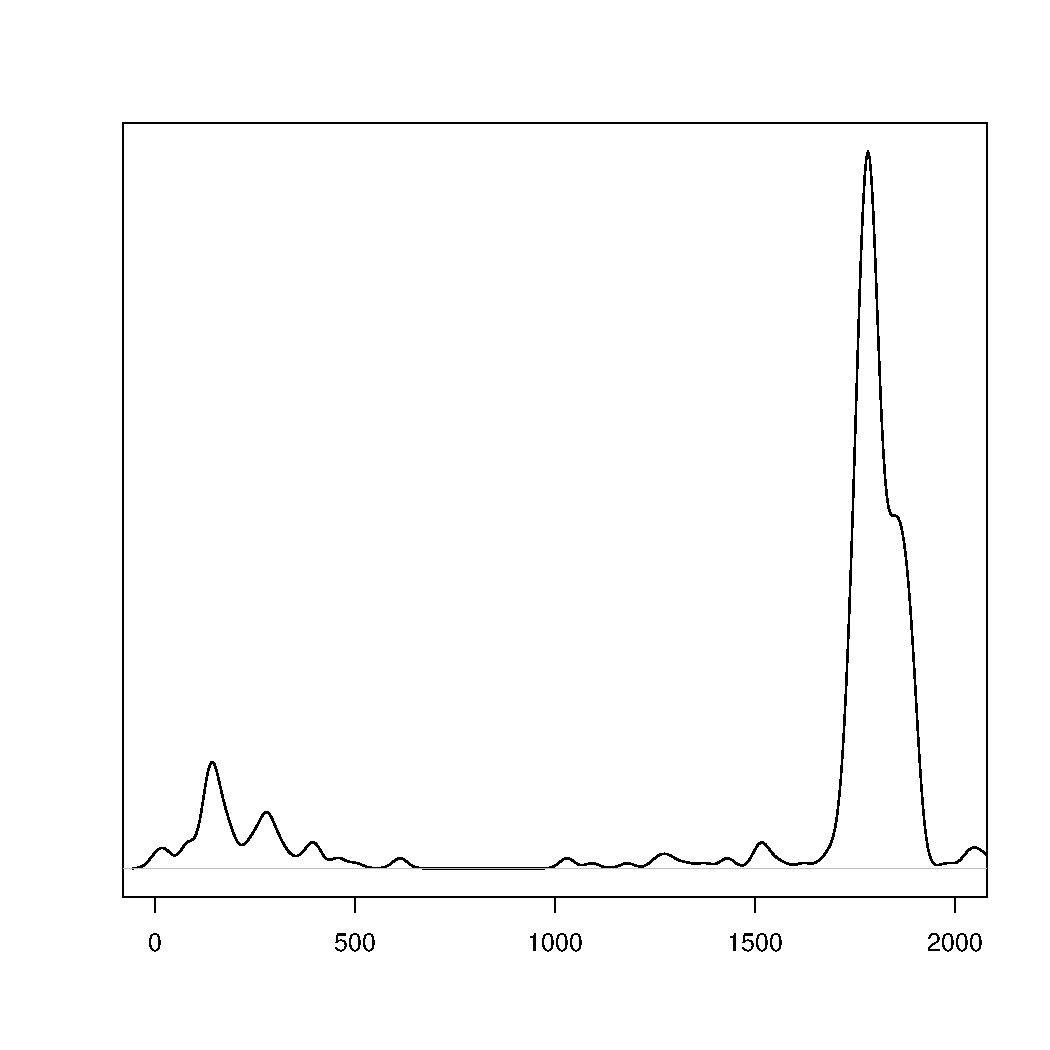
\includegraphics[width=4cm]{analysis/301/301-trec8.pdf}
\caption{All}
\end{subfigure}
\begin{subfigure}[t]{4cm}
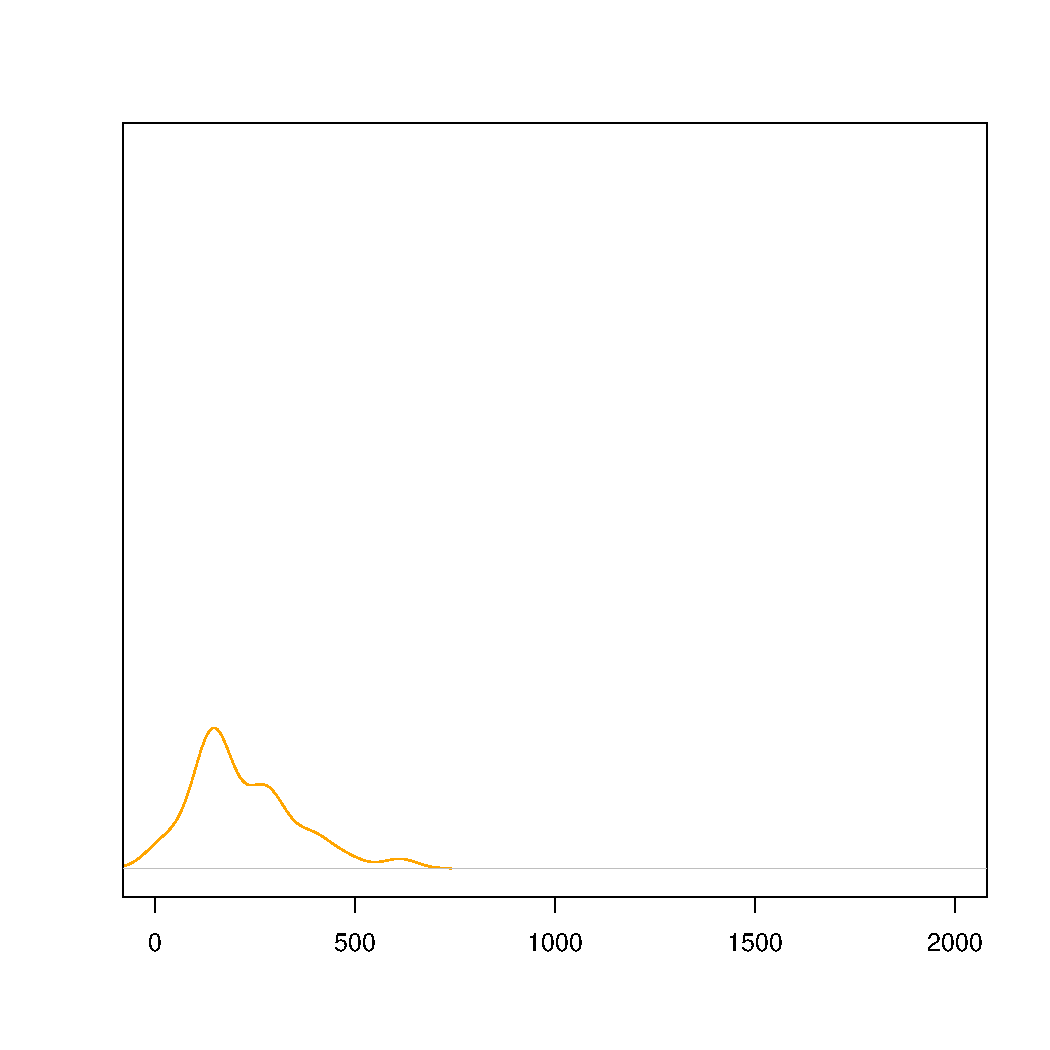
\includegraphics[width=4cm]{analysis/301/301-la.pdf}
\caption{LA Times}
\end{subfigure}
\begin{subfigure}[t]{4cm}
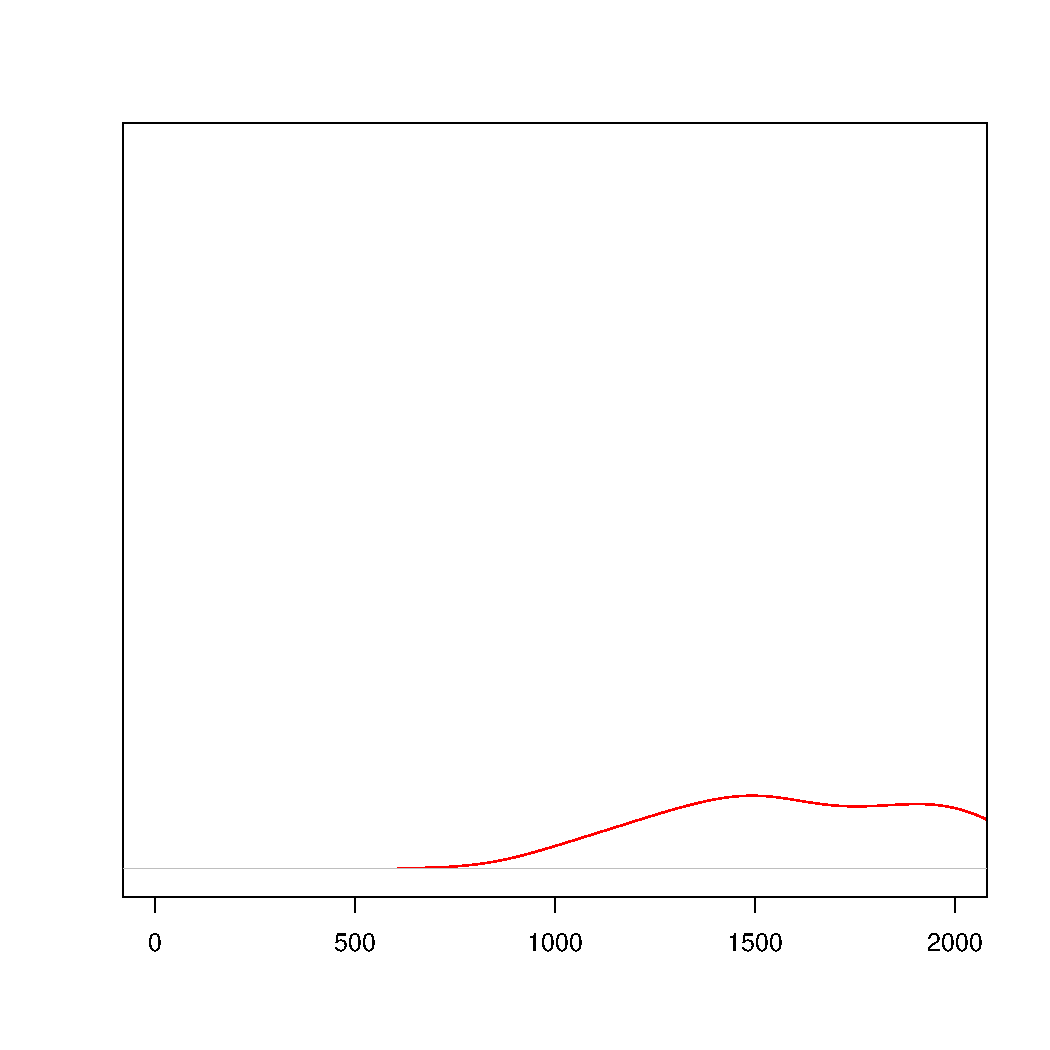
\includegraphics[width=4cm]{analysis/301/301-ft.pdf}
\caption{FT}
\end{subfigure}
\begin{subfigure}[t]{4cm}
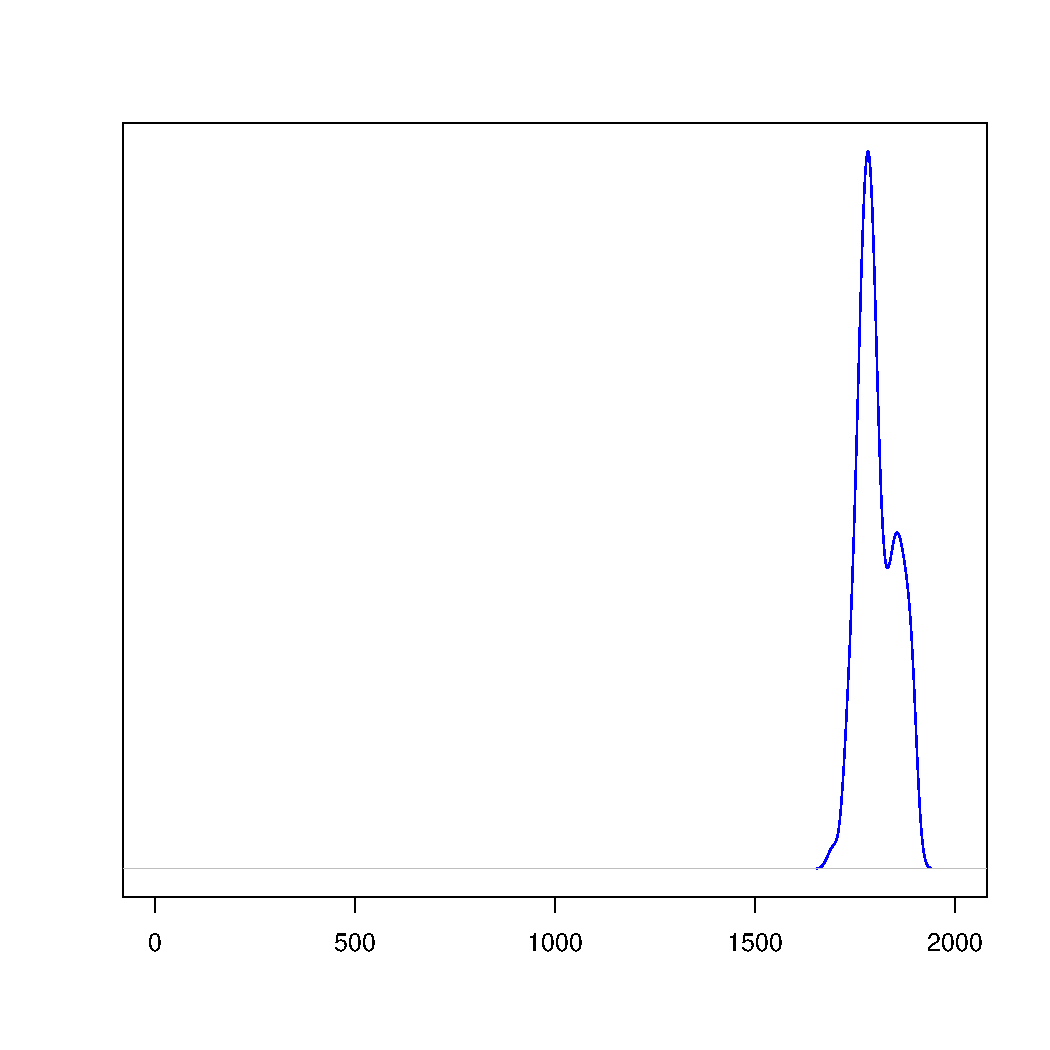
\includegraphics[width=4cm]{analysis/301/301-fbis.pdf}
\caption{FBIS}
\end{subfigure}
\caption{Temporal distribution of relevant documents for topic 301 by sub-collection} 
\label{fig.301}
\end{figure}


We propose a few principles to guide future work on the evaluation of temporal retrieval models. We plan to explore this in future work.

Aside from the Novelty track topics, the other manual classifications consistently conflate two different concepts: the temporal distribution of judged-relevant documents and a common-sense notion of topic temporality. The temporal distribution of judged-relevant documents is an important indicator of possible temporality, particularly as models often rely on pseudo-relevant document distributions in scoring. However, these distributions alone are not adequate, which is why common-sense criteria have been introduced to determine whether topics have ``bona-fide temporal dimensions'' \cite{Efron2011}. We recommend considering these two concepts separately.  Since the first-order autocorrelation of the judged-relevant document distribution is highly correlated with manual judgements of temporality, we suggest  using this or another measure of distribution ``burstiness'' or ``peakedness'' instead of manual assessment to improve repeatability.

Common-sense notions of temporality should be clearly explicated.  We found that the presence of different classes of events, as captured in the qualitative codes, would seem to be strong indicators of topic temporality.  This is the case in the Novelty and Blog classifications. As suggested in Figure \ref{fig.codedist}(c), topics 301-450 have fewer specific events, similar to the findings of Jones and Diaz with the AP and WSJ collections. This suggests that the earlier TREC test collections, including TREC8, may not be well-suited to temporal retrieval research because of the nature of the topics. These collections are also problematic because of different temporal characteristics of individual sub-collections.

Sub-collections should be considered independently. Each sub-collection has different temporal dimensions (start/end dates), topical coverage, and document volumes. By combining sub-collections for temporal analysis, researchers risk falsely identifying temporally-sensitive queries. An example is given in Figure \ref{fig.301}, which breaks down the distribution of relevant documents by sub-collection in TREC8 for query 301 (international organized crime). This query was used as an exemplar of recency queries by Li and Croft \cite{Li2003}. Looking at the distribution across all of TREC8 (3a), this would appear to be a recency query, since more relevant documents are found toward the end of the collection. However, broken down by sub-collection, we see that this is due to a high number of judged relevant documents in FBIS. Though the FT subcollection contains relevant documents during the same time frame as the FBIS spike, the peakedness of that subcollection is significantly less, suggesting considerable differences in the makeup of FT and FBIS. In fact, many of the recency queries in Li and Croft have large numbers of relevant documents in the FBIS sub-collection.  This leads us to recommend that individual sub-collections should be considered independently. Due to this problem, future researchers should recognize the limits of  Li and Croft's classified queries.

Using individual sub-collections can sometimes be problematic. For example,  the LA Times and Financial Times sub-collections have surprisingly few judged-relevant documents. The LA Times has an average of 24 and Financial Times 33 judged-relevant documents per topic.  Using Dakka et al's \cite{Dakka2012} criterion of $>20$ judged-relevant documents per topic for the assessment of temporality, only 53 and 70 topics respectively would be available for analysis. This again suggests that the TREC8 sub-collections are not well-suited for this type of temporal retrieval research.

Returning to the NTCIR Temporalia collection, researchers should be clear about the distinction between \emph{temporal relevance} and \emph{temporal topicality} in the creation of test collections. While highly related, these concepts are distinct. Models temporal topicality are unlikely to be effective when measuring temporal relevance and vice-versa.

\section{Conclusion}

Through the in-depth analysis of test collections developed for temporal IR research, we have identified a number of complexities underlying the classification of temporally sensitive queries, suggesting new approaches to incorporating time into retrieval models and test collections. We also found that topics related to specific and periodic events are promising indicators of temporal sensitivity that have not yet been fully explored.  

In future work, we intend to expand this study to consider additional test collections, including those for the more recent filtering tracks \cite{Frank2013, Guo2013}. We also plan to further explore the role of ``events'' in temporal retrieval models.

\section{Acknowledgments}
This work was supported in part by the US National Science Foundation under Grant No. [blind]. Any opinions, findings, conclusions, or recommendations expressed are those of the authors and do not necessarily reflect the views of the National Science Foundation. 

\bibliographystyle{abbrv}
\bibliography{temporalir}  

\end{document}
